\documentclass{beamer}
\usepackage[autokw=all]{svn-multi}
\setbeamertemplate{navigation symbols}{}
%\usetheme{Goettingen}
\usetheme{Malmoe}
\usefonttheme{default}

\usepackage{hyperref}
\usepackage{subfigure}
\usepackage{amsmath}
\usepackage{amssymb}
\usepackage{multimedia}
\usepackage{shadow}
%\usepackage{movie15}

%\usepackage[english]{babel}
%\usepackage{pgf,pgfarrows,pgfnodes,pgfautomata,pgfheaps}
% \usepackage[latin1]{inputenc}

\usepackage{graphicx}
\defbeamertemplate*{footline}{default theme}
{
  \leavevmode%
  \hbox{%
  \begin{beamercolorbox}[wd=.5\paperwidth,ht=2.25ex,dp=1ex,center]{author in head/foot}%
    %\usebeamerfont{author in head/foot}\insertshortauthor~~(\insertshortinstitute)
    \usebeamerfont{author in head/foot}\insertshortauthor
  \end{beamercolorbox}%
  \begin{beamercolorbox}[wd=.4\paperwidth,ht=2.25ex,dp=1ex,center]{title in head/foot}%
    \usebeamerfont{title in head/foot}\insertshorttitle
  \end{beamercolorbox}%
  \begin{beamercolorbox}[wd=.1\paperwidth,ht=2.25ex,dp=1ex,right]{date in head/foot}%
%    \usebeamerfont{page number}\insertframenumber{} / \inserttotalframenumber\hspace*{2ex} 
    \usebeamerfont{page number}\insertpagenumber{} / \insertpresentationendpage{} \hspace*{2ex} 
  \end{beamercolorbox}}%
  \vskip0pt%
}

\title{Software for Mind Control}

\author{Ben Pearre}
%\institute[]{
%  Computer Science\\
%  University of Colorado at Boulder, USA}
\date{\today\\{\small (Rev. \svnrev)}}
%\date{\today}

\begin{document}

\begin{frame}
  \titlepage
\end{frame}

\begin{frame}
  \frametitle{Outline}
  \tableofcontents
\end{frame}


%\begin{frame}
%  \outline
%\end{frame}

%%% Syllable Detector %%%
\section{Syllable detector}
\subsection{Goals}

\begin{frame}
  \frametitle{Syllable Detector}
  \begin{columns}
    \column{5cm}
    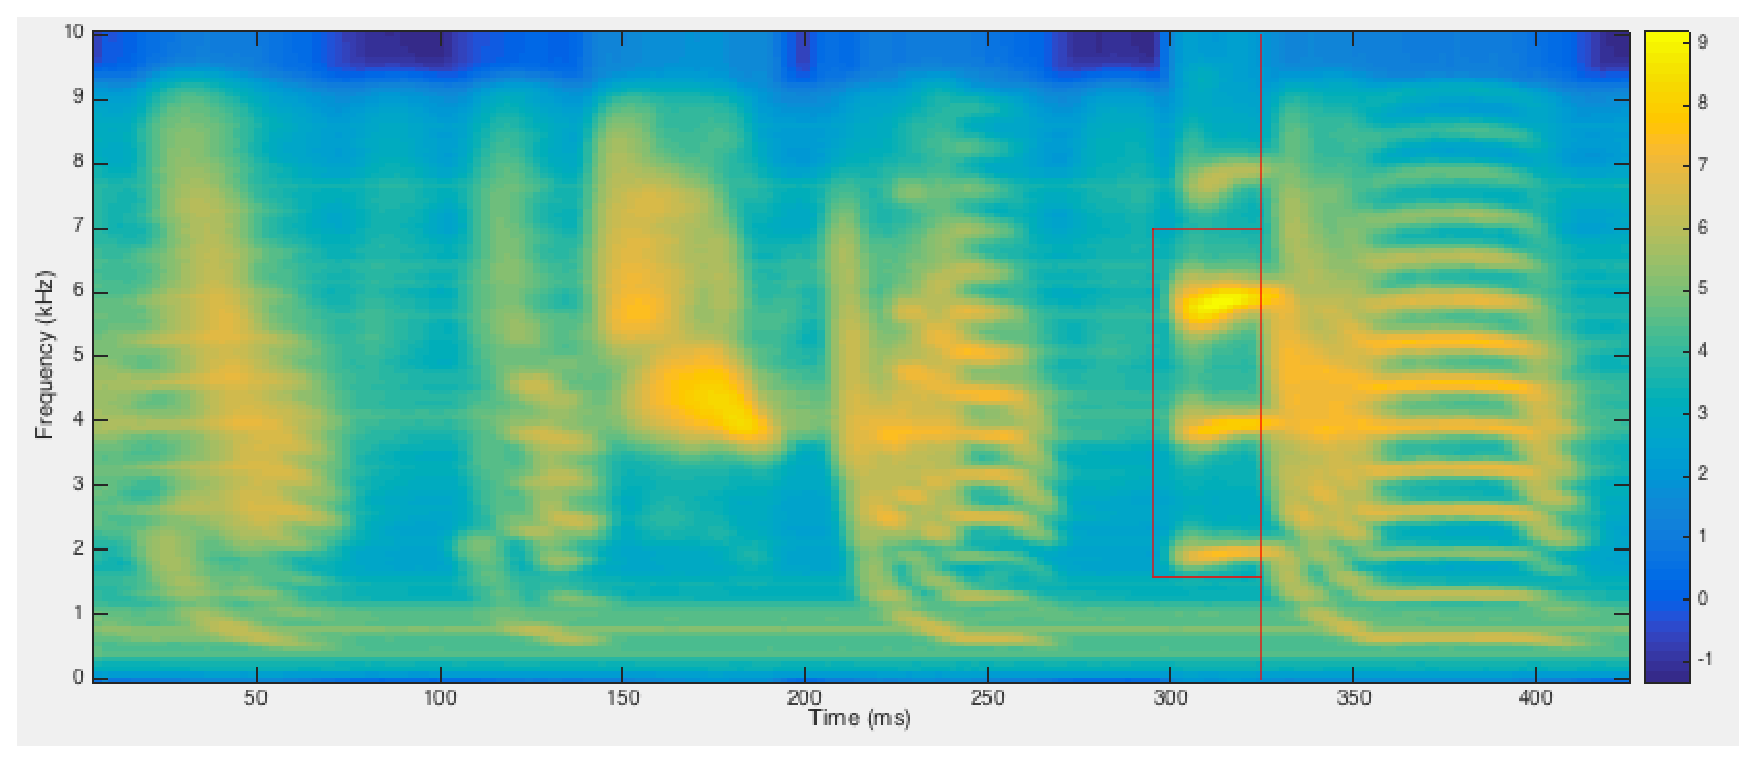
\includegraphics[width=5cm]{song-spectrogram-with-alignment-1}
    \column{50mm}
    Goals:
    \begin{itemize}
    \item Detect any point in song?
    \item Best accuracy
    \item Low latency
    \item Low jitter
    \end{itemize}
  \end{columns}
\end{frame}

\subsection{Workflow}

\begin{frame}
  \frametitle{Jeff's song alignment}
  Install from {\tt https://github.com/jmarkow}:
  \begin{itemize}
    \item {\tt ephys}
    \item {\tt markolab}
    \item {\tt zftftb}
    \item {\tt robofinch}
  \end{itemize}
  Workflow---using {\tt zftftb\_song\_clust.m}:
  \begin{itemize}
    \item Select template syllable
    \item Cluster
  \end{itemize}

  \noindent Align about 500 songs.
  \begin{description}
    \item[Input:] Raw recordings
    \item[Output:] A Matlab file of aligned songs
  \end{description}
\end{frame}

\begin{frame}
  \frametitle{Ben's song detection}
  Install from {\tt https://github.com/bwpearre}:
  \begin{itemize}
    \item {\tt birds}
  \end{itemize}
  Load {\tt birds/align/learn\_detector.m}:

  \begin{description}
    \item[Input:] a file of aligned songs.
    \item[Output:]
      \begin{itemize}
      \item neural network file
      \item audio testing file
      \end{itemize}
  \end{description}
      
\end{frame}

\begin{frame}
  \frametitle{Choose a moment during song}
  Tune some parameters\dots

  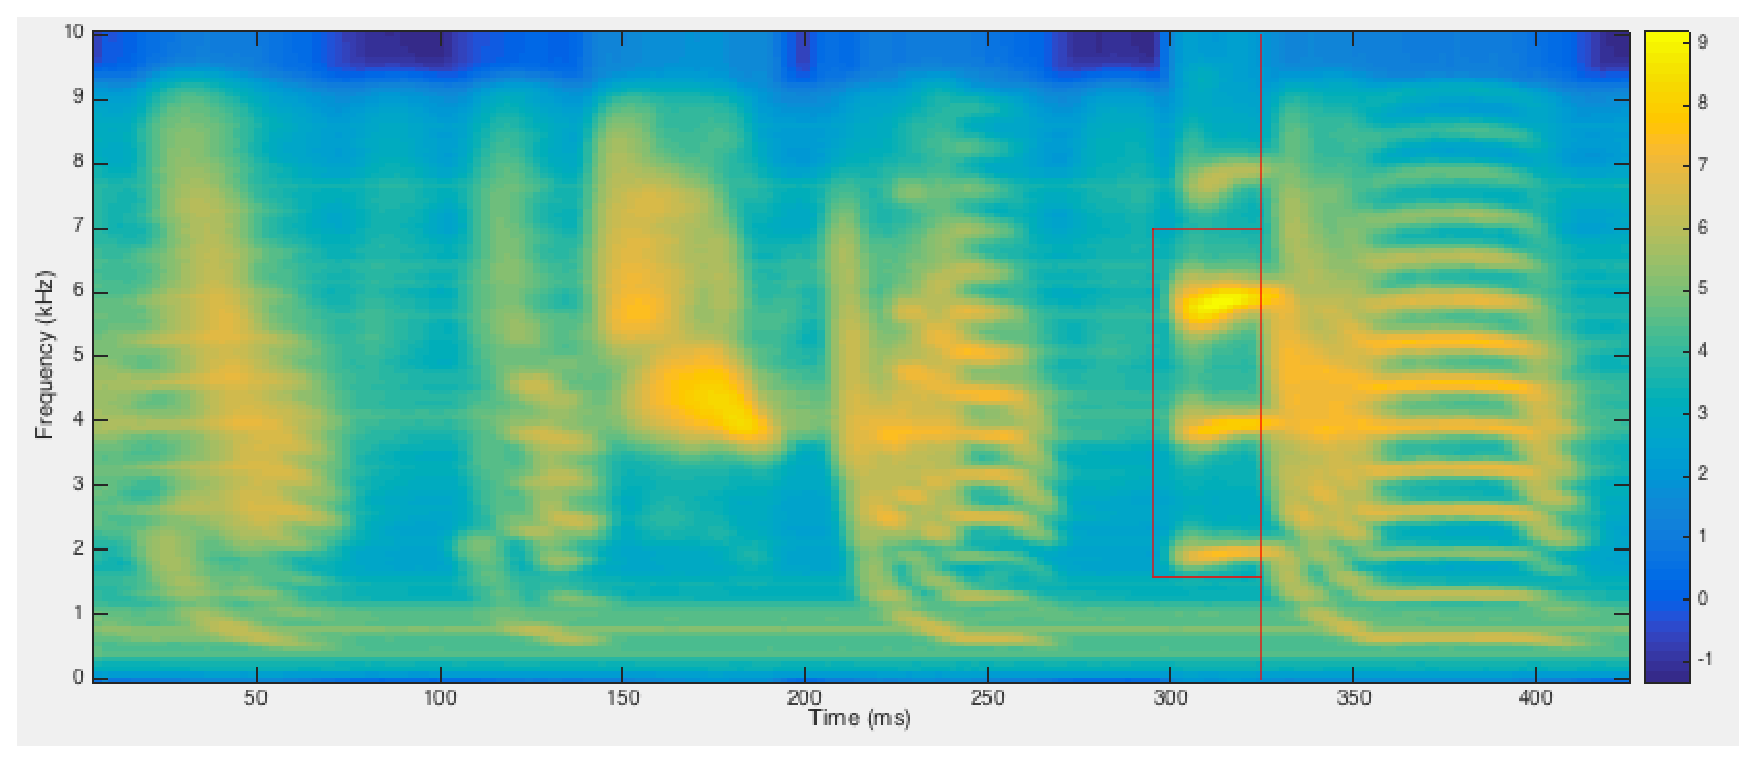
\includegraphics[width=11cm]{song-spectrogram-with-alignment-1}

  Run it\dots
\end{frame}

\begin{frame}
  \frametitle{LabView interface}

  \includegraphics<1>[width=11cm]{labview-spaghetti}
  \includegraphics<2>[width=11cm]{labview-frontend}

  \begin{description}
    \item[Input:] Neural network file\dots
    \item[Output:] TTL pulses etc\dots
  \end{description}
\end{frame}

%%%%%%%%%%%%%%%%
\subsection{Results}

\begin{frame}
  \frametitle{Detection}
  \begin{center}
    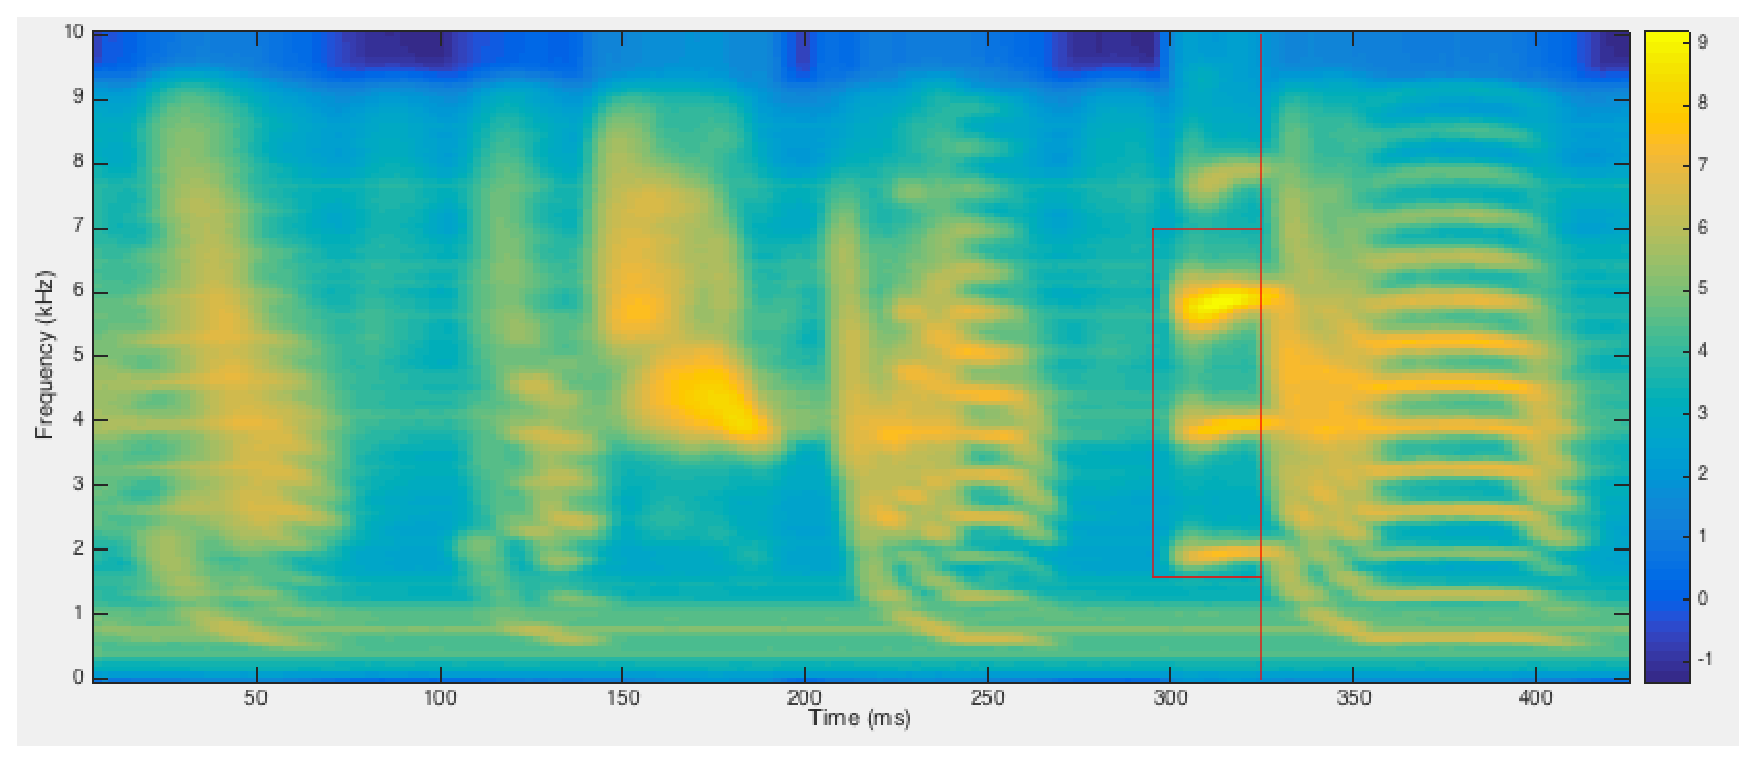
\includegraphics[width=8cm]{song-spectrogram-with-alignment-1}
  \end{center}
  \par
  \begin{center}
    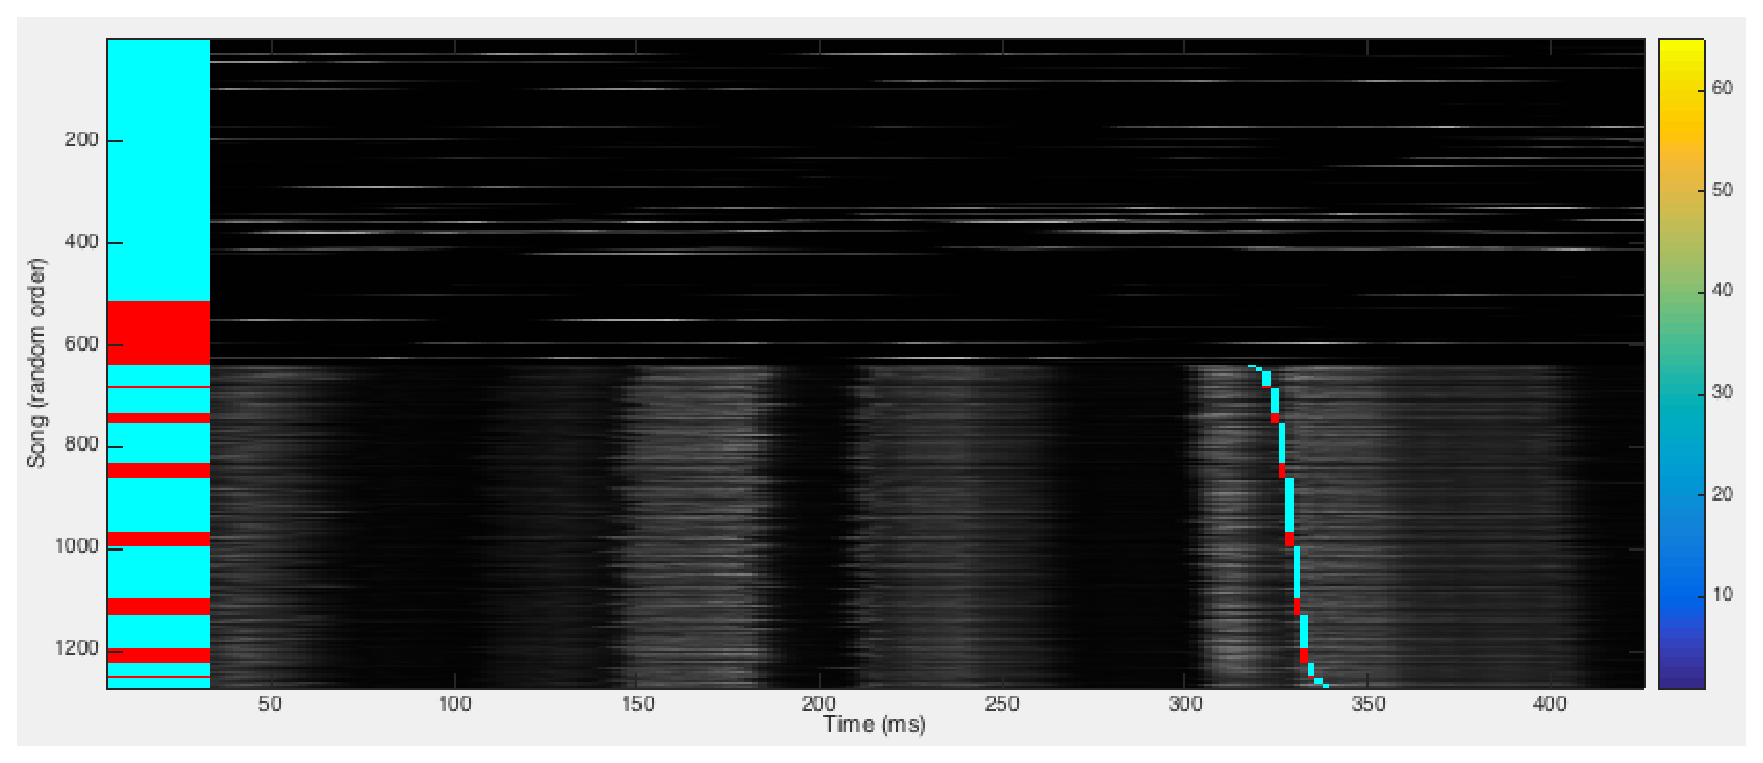
\includegraphics[width=8cm]{song-spectrogram-with-alignment-2}
  \end{center}
\end{frame}

\begin{frame}
  \frametitle{Detection}
  \includegraphics<1->[width=\textwidth]{syllablebank-0}
  \par
  \includegraphics<2>[width=\textwidth]{syllablebank-1}
  \includegraphics<3>[width=\textwidth]{syllablebank-2}
  \includegraphics<4>[width=\textwidth]{syllablebank-3}
  \includegraphics<5>[width=\textwidth]{syllablebank-4}
  \includegraphics<6>[width=\textwidth]{syllablebank-5}
  \includegraphics<7>[width=\textwidth]{syllablebank-6}
  \includegraphics<8>[width=\textwidth]{syllablebank-roc}
\end{frame}

\begin{frame}
  \begin{center}
    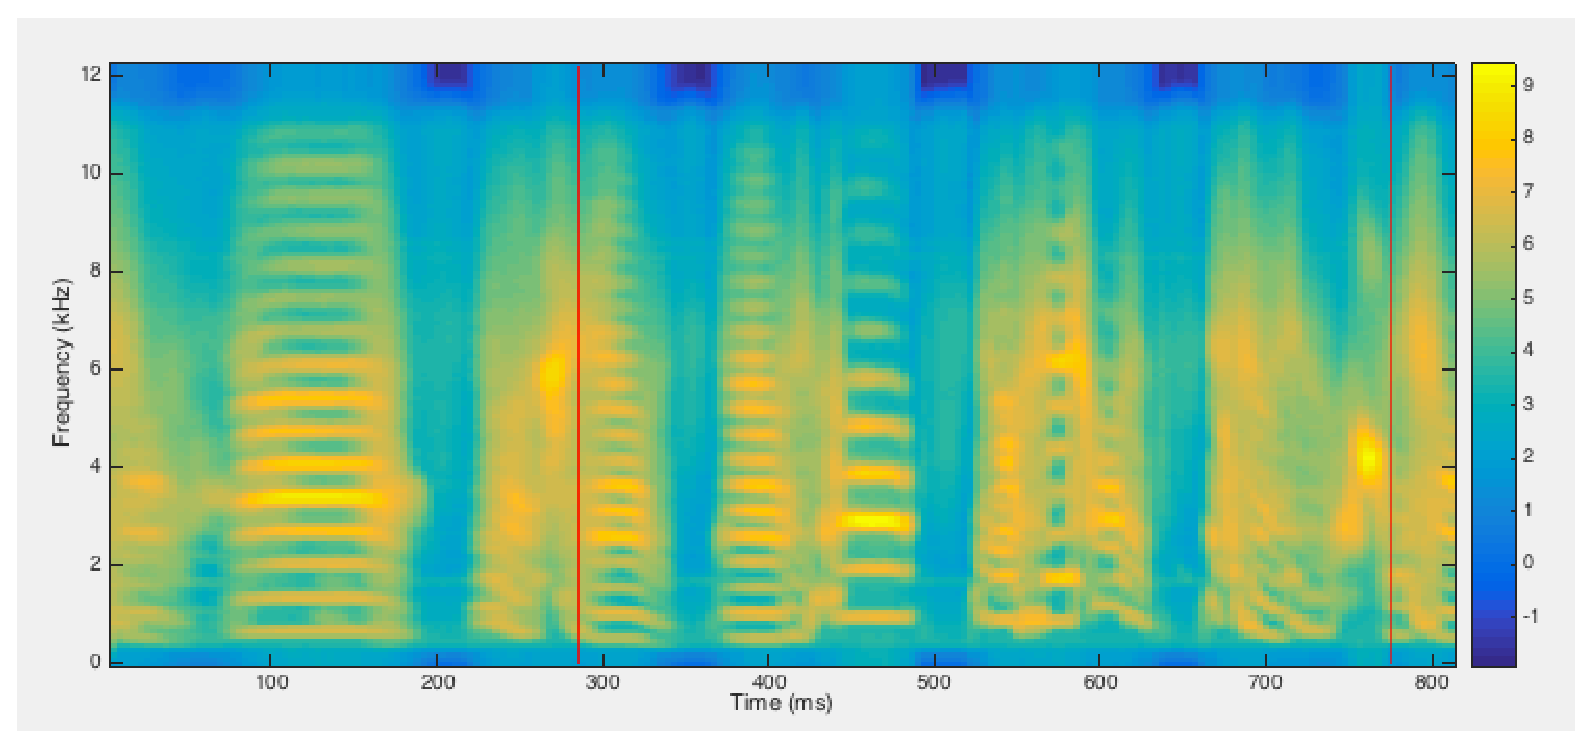
\includegraphics[width=8cm]{detector2-spectrogram}
  \end{center}
  \par
  \begin{center}
    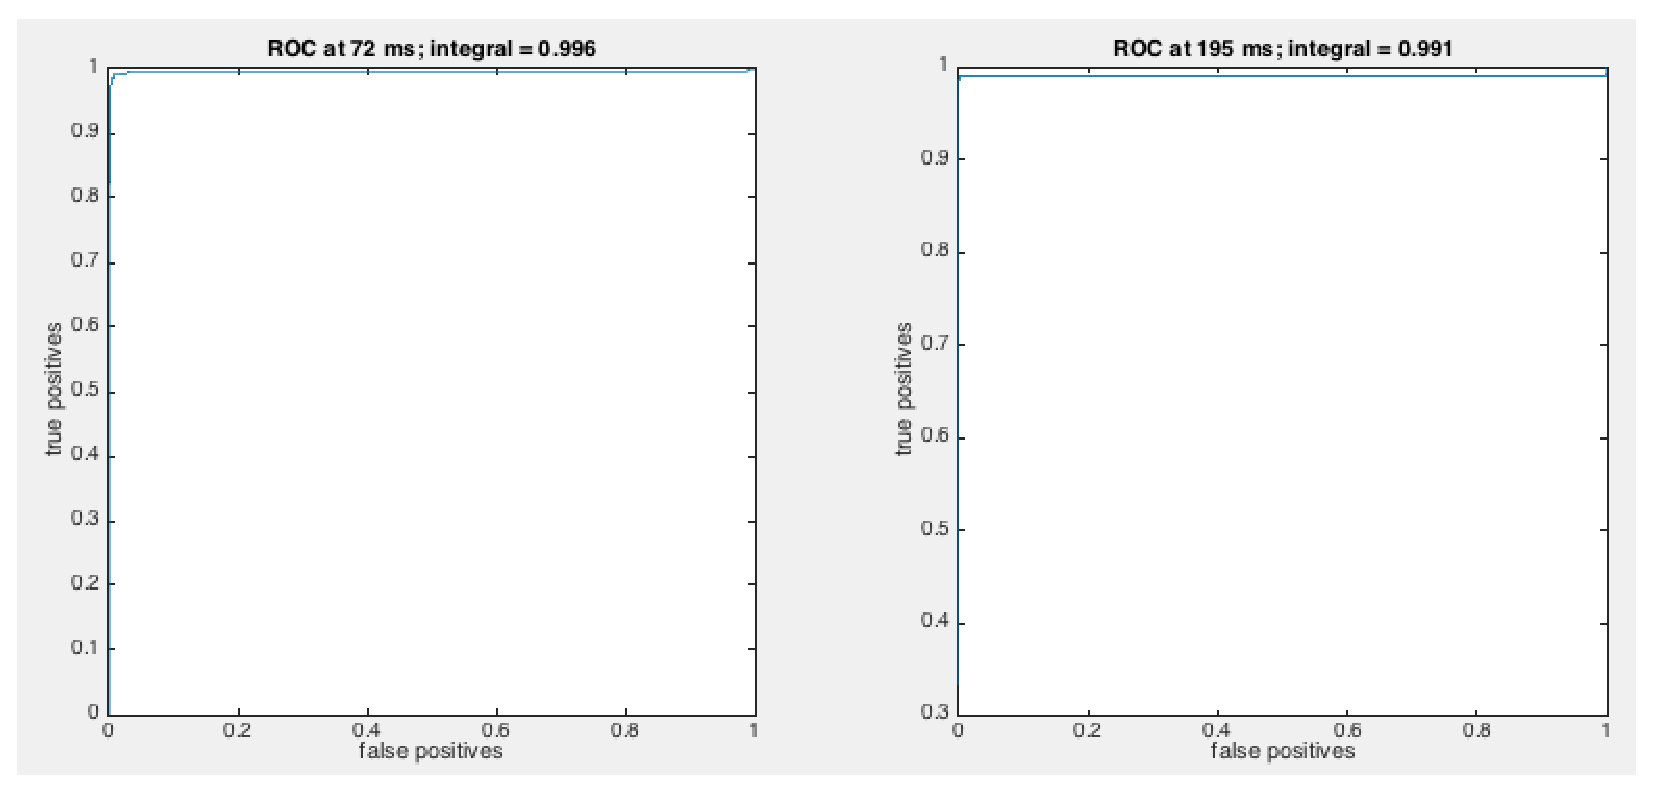
\includegraphics[width=6cm]{detector2-roc}
  \end{center}
\end{frame}


\begin{frame}
  \frametitle{Testing: timing}
  \includegraphics[width=8cm]{detector-timing-1}
\end{frame}

\begin{frame}
  \frametitle{Testing: timing}
  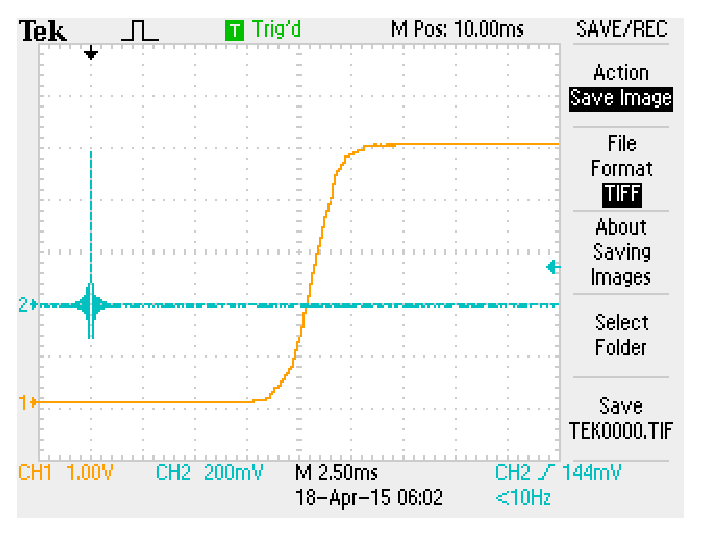
\includegraphics[width=8cm]{detector-timing-2}
\end{frame}

\subsection{Current status}

\begin{frame}
  \frametitle{Current status}
  \begin{itemize}
    \item Matlab has high accuracy!
    \item Labview: lower accuracy.  Bug?
    \item Inferior song detector
    \item Nathan?
  \end{itemize}
\end{frame}


%%% Win's Work %%%
\section{Stimulation}
\subsection{Goals}

\begin{frame}
  \frametitle{Goals}
  \begin{itemize}
  \item Modify neural signals
    \begin{itemize}
    \item CNS
    \item Peripheral --- Win!
    \end{itemize}
  \item Optimise pulse shapes
  \item Develop control policies to systematically modify behaviours
  \end{itemize}
\end{frame}


\subsection{Tools --- hardware}

\begin{frame}
  \frametitle{Electrodes}
  Chronic high-count low-impedance\dots
  \begin{itemize}
    \item Carbon fibres
    \item Carbon nanotubes
    \item Silicon carbide
  \end{itemize}
  Simultaneous stimulation and recording may require\dots {\em optical?}
\end{frame}

\begin{frame}
  \frametitle{Plexon stimulator}
  \begin{itemize}
    \item Current-controlled
    \item Arbitrary pulse waveforms
    \item 30 nA resolution
    \item 16 independent channels
    \item Matlab API
    \item Reprogramming time $\simeq$ 0.05s/channel
  \end{itemize}
\end{frame}
    

\begin{frame}
  \frametitle{Recording amplifiers}
  \begin{columns}
    \column{33mm}
    Intan
    \begin{itemize}
      \item $\geq$ 16 channels
      \item Easy impedance measurements
      \item Low noise
      \item {\it Very poor blanking}
        \begin{itemize}
        \item artifacts at $>$ 3ms
        \end{itemize}
    \end{itemize}
    \column{33mm}
    A M Systems
    \begin{itemize}
      \item 2 or 4 channels per amp
        \begin{itemize}
          \item (Connectivity?)
        \end{itemize}
      \item Difficult to do impedance measurements
      \item Headstages need to be built
      \item Few artifacts
    \end{itemize}
    \column{33mm}
    TDT
    \begin{itemize}
      \item $\geq$ 16 channels
      \item No impedance measurements
      \item Low noise
      \item Few artifacts
      \item Talks to Matlab
      \item Quirky.  Buggy.
      \item \dots oh, and it's also a DSP!
    \end{itemize}
  \end{columns}
\end{frame}

\subsection{Tools --- software}

\begin{frame}
  \frametitle{{\tt plexme}}
  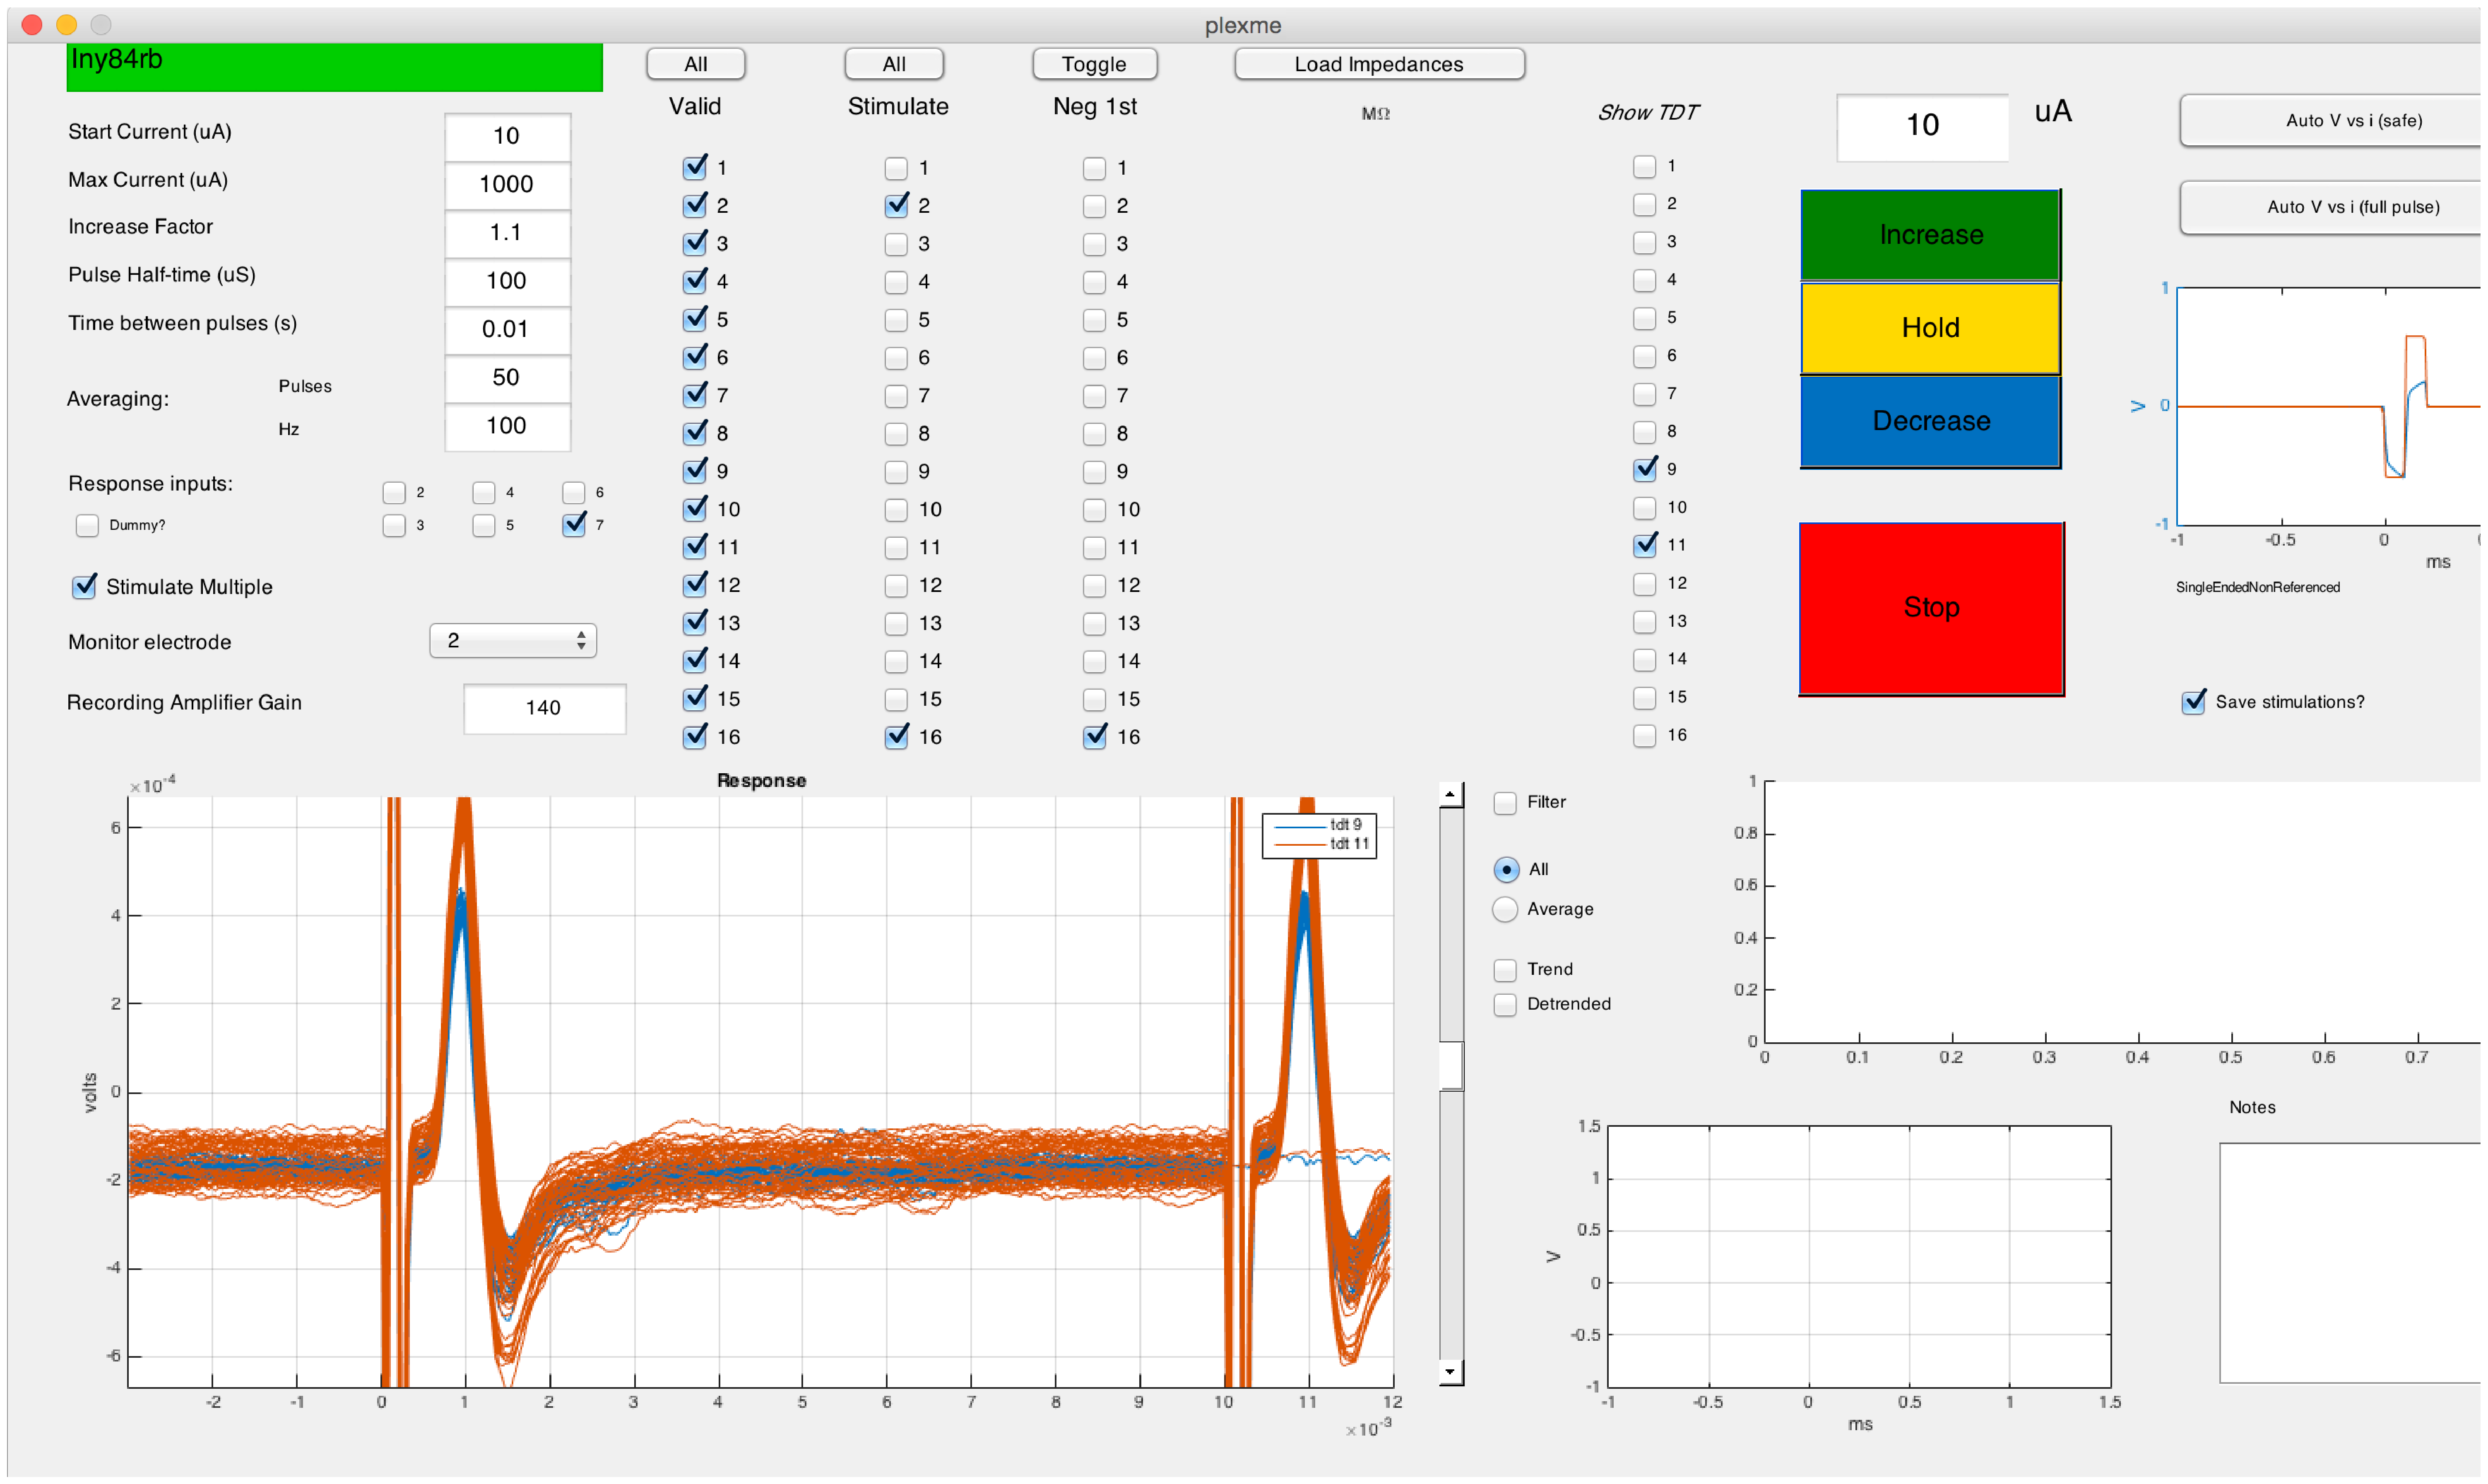
\includegraphics[width=\textwidth]{plexme-faked}
\end{frame}

\begin{frame}
  \frametitle{{\tt inspect}}
  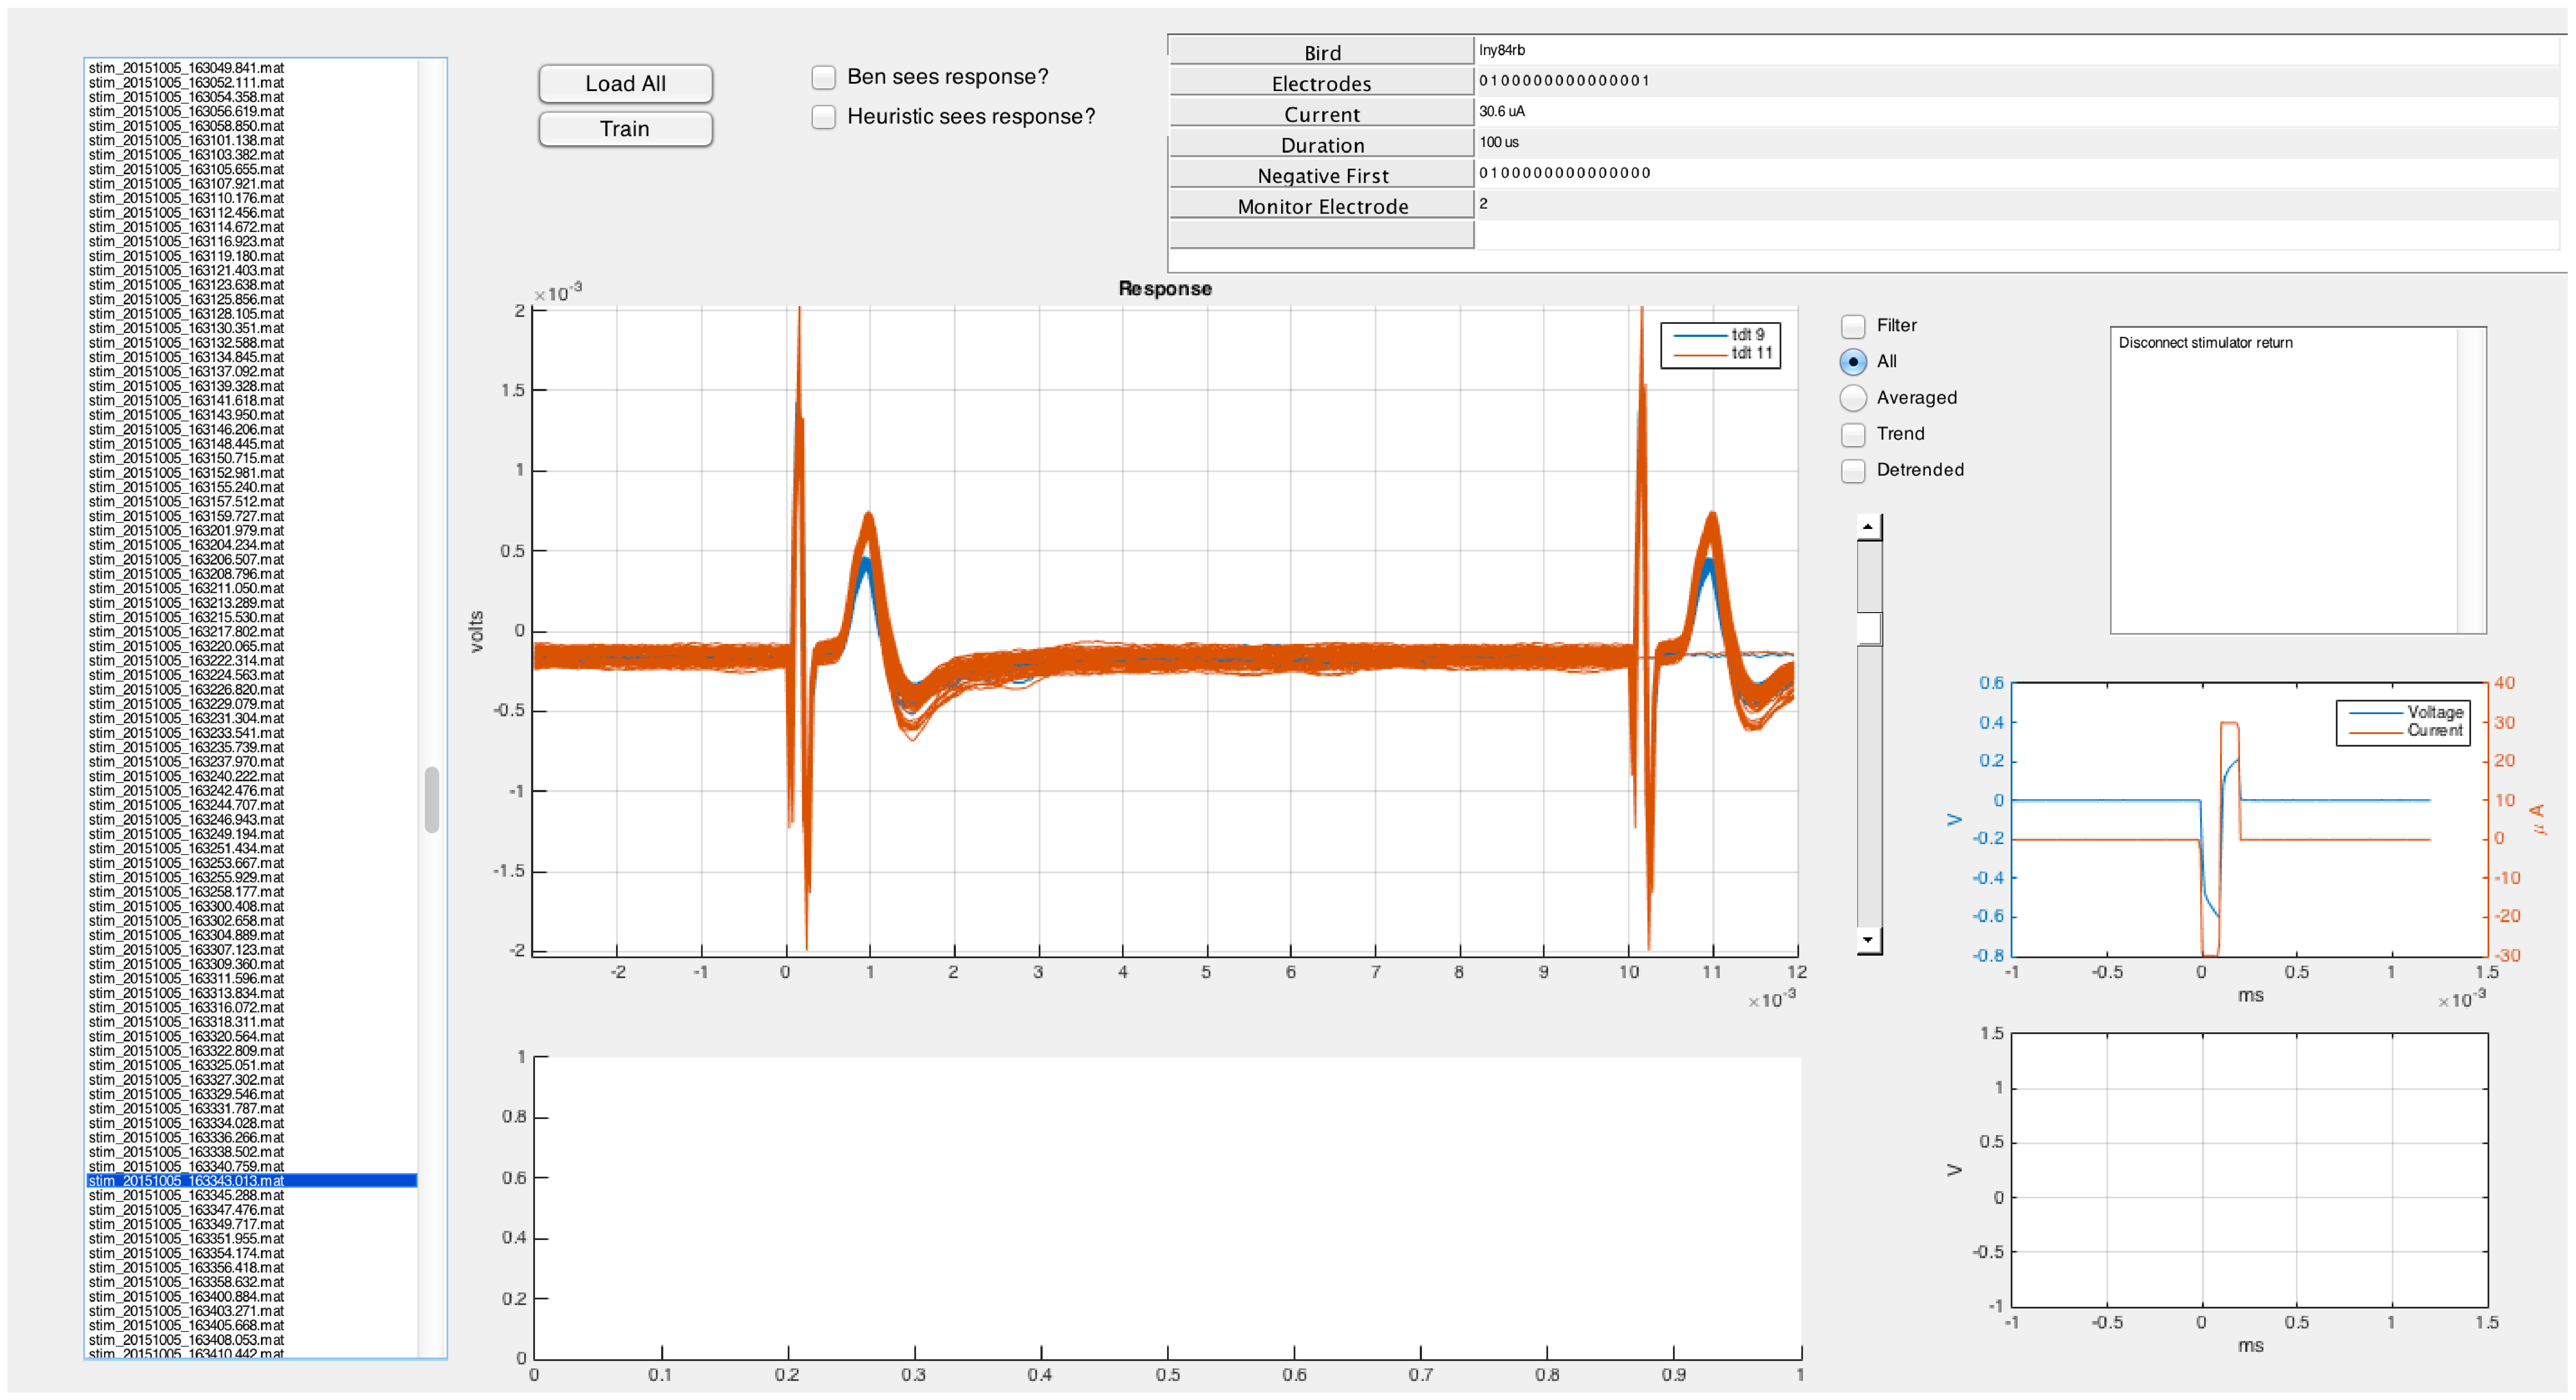
\includegraphics[width=\textwidth]{inspect-example-1}
\end{frame}


\subsection{Results}

\begin{frame}
  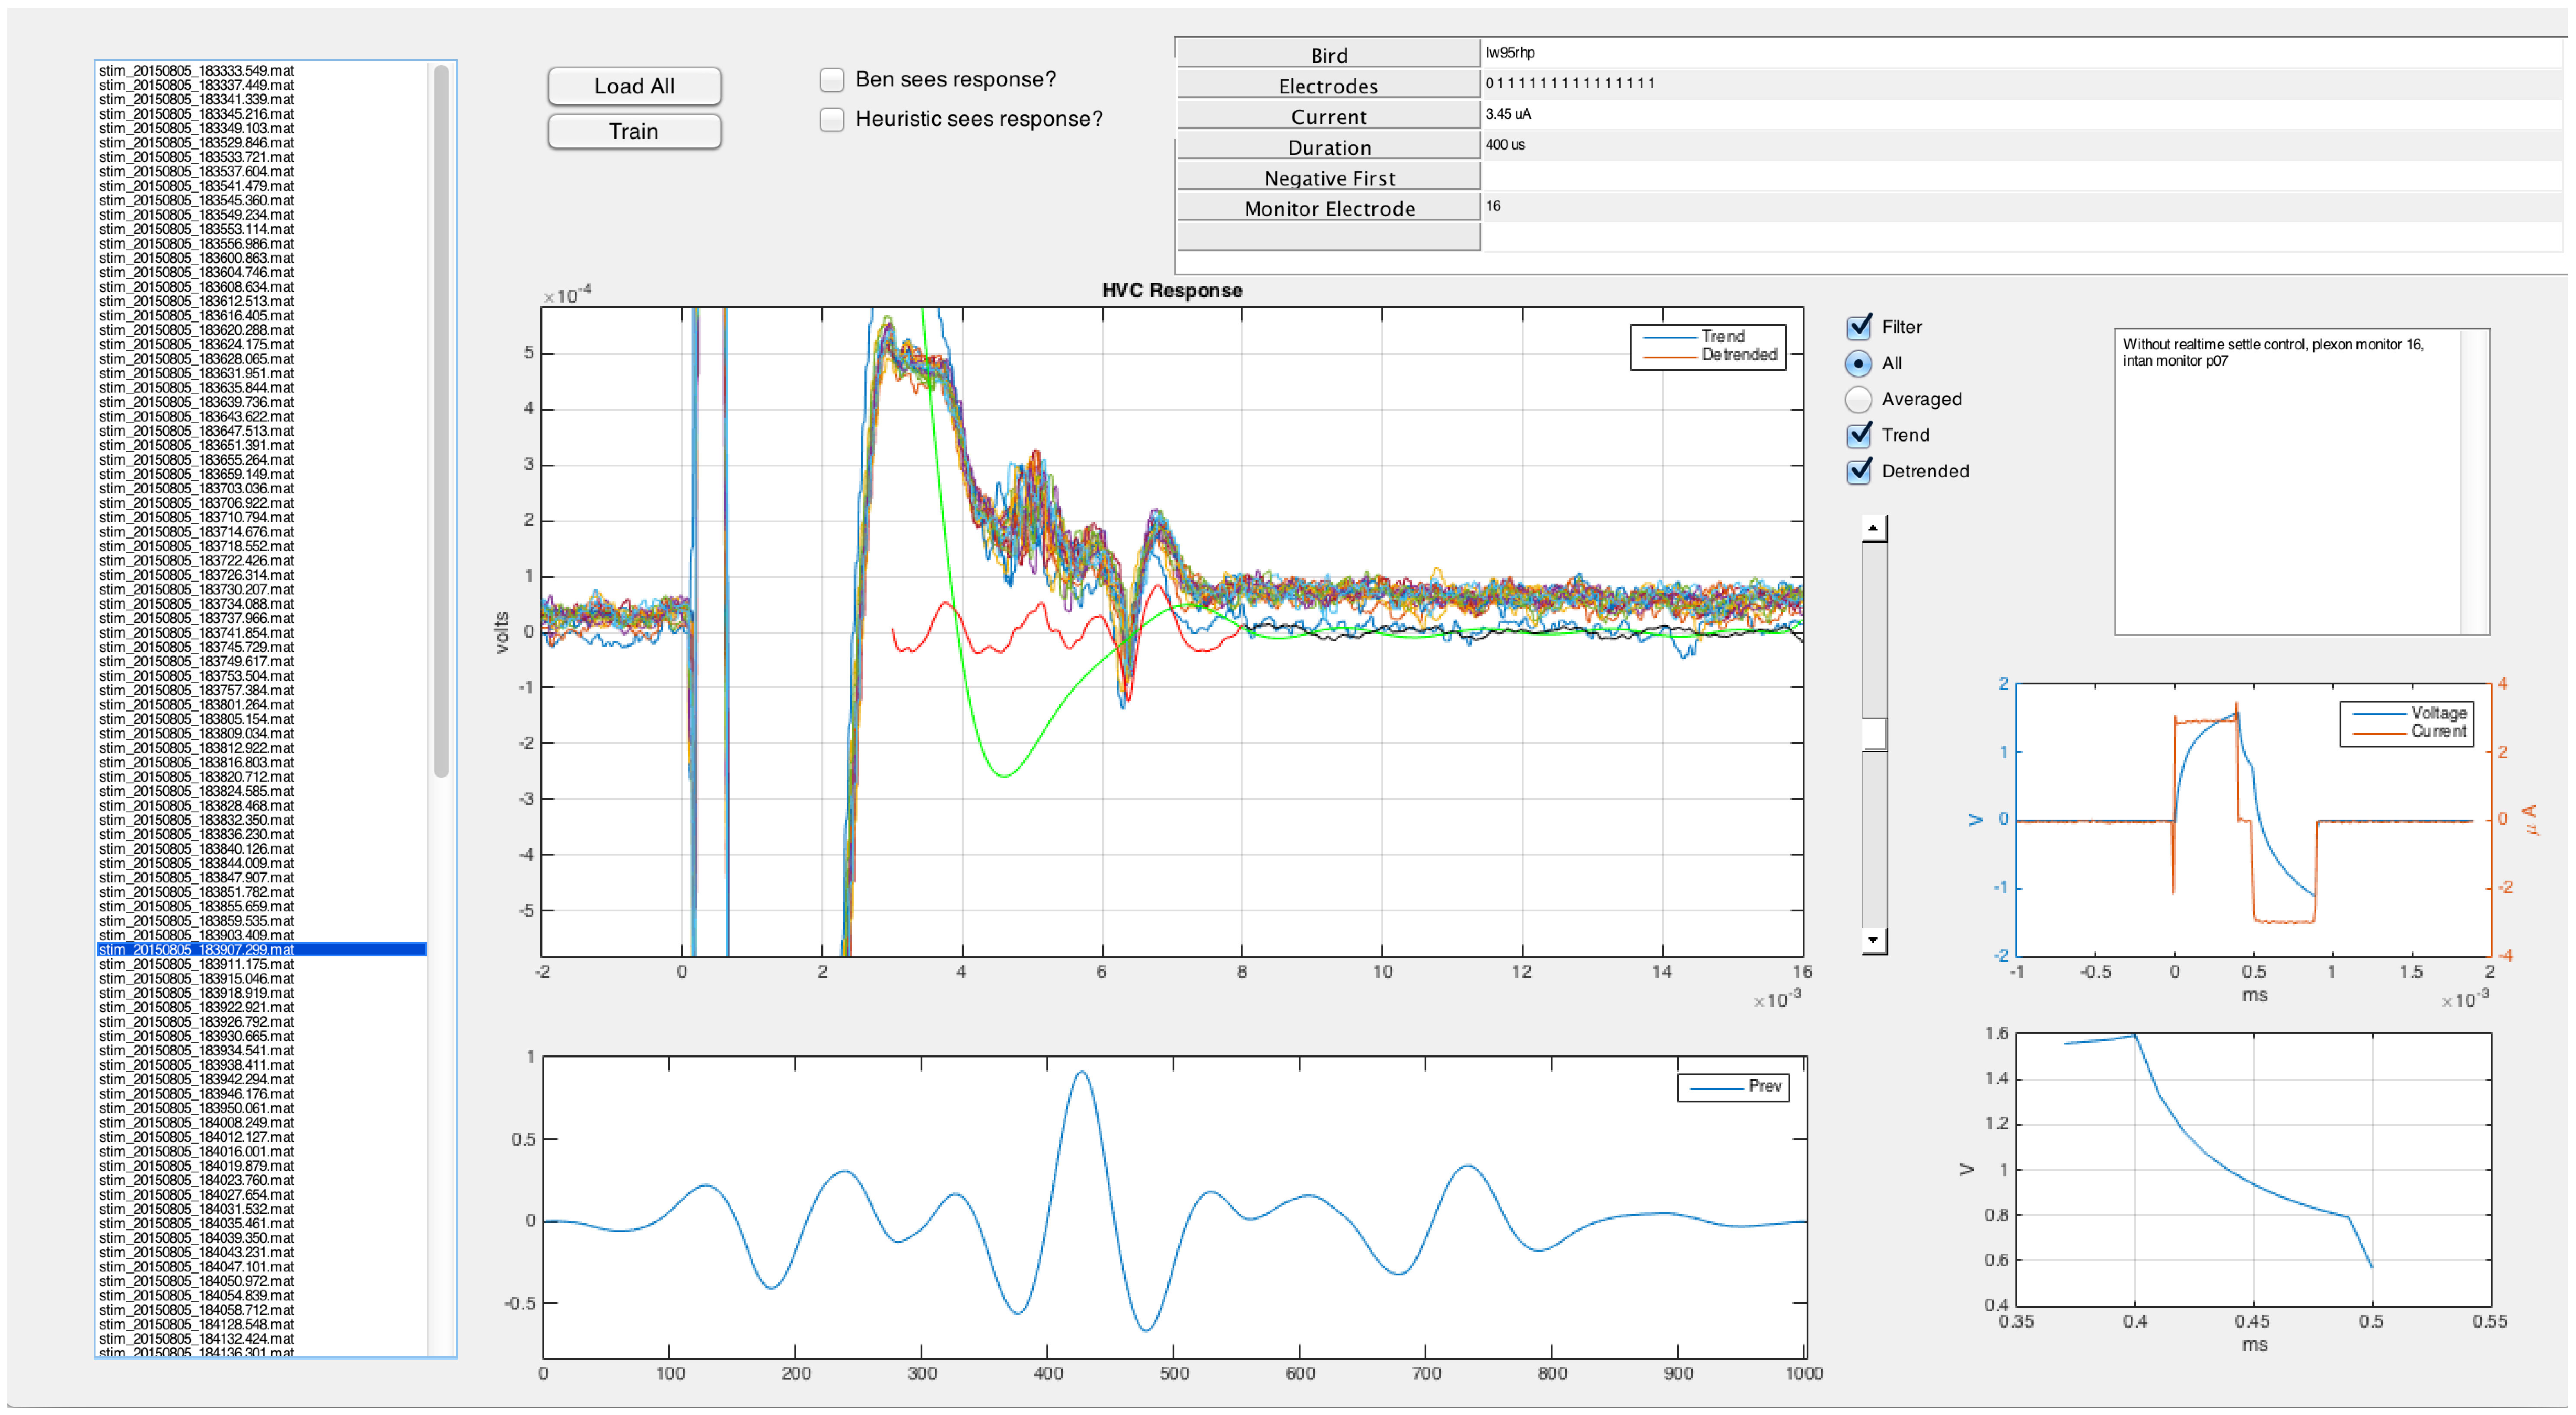
\includegraphics[width=\textwidth]{inspect-example-0}
\end{frame}

%%% Future! %%%
\section{The Future!}
\subsection{Goals}

\begin{frame}
  \frametitle{Goals}
  \begin{itemize}
    \item Optimise stimulation
      % What optimisation criteria?
      % What policy variables?
      % What model?  Canary?
  \end{itemize}
\end{frame}

\subsection{Approach}

\begin{frame}
  \frametitle{Stochastic Optimisation}
\end{frame}

\begin{frame}
  \frametitle{Reinforcement Learning}
\end{frame}

\subsection{Timeline}



\end{document}
